\chapter{Alta disponibilidade}
\label{cap:altadiponibilidade}

Alta disponibilidade é muito conhecida, sendo cada vez mais empregada nos ambientes computacionais. O objetivo de promover alta disponibilidade 
resume-se em garantir que um serviço esteja sempre a disposição quando o cliente solicitar ou acessar \cite{costa2009}.
A alta disponibilidade é definida como a redundância de \textit{hardware} ou \textit{software} para que o serviço fique mais tempo disponível.
Quanto maior for a disponibilidade desejada maior deverá ser a redundância no ambiente, assim reduzindo os pontos únicos de falha,
que em inglês são chamados de \textit{Single Point Of Failure} (SPOF).

A alta disponibilidade está diretamente relacionada a dependabilidade, confiabilidade, disponibilidade e tolerância a falhas. 
\begin{itemize}
 \item Dependabilidade indica a qualidade do serviço fornecido e a confiança depositada nele. A dependabilidade envolve vários
atributos como segunrança de funcionamento, segurança, manutenabilidade, testabilidade e comprometimento do desempenho \cite{weber2002};
 \item Confiabilidade é o mais importante atributo, pois transmite a ideia de continuidade de serviço \cite{pankaj1994}. A confiabilidade refere-se 
a probabilidade de um serviço funcionar corretamente durante um dado intervalo de tempo. Já a disponibilidade é a probabilidade de um 
serviço estar operacional no instante em que for solicitado \cite{costa2009};
  \item Tolerância a falhas tenta garantir a disponibilidade de um serviço utilizando mecanismos capazes de detectar, mascarar e recuperar falhas, 
e seu objetivo é alcançar a dependabilidade, assim indicando uma boa qualidade de serviço \cite{costa2009}.
\end{itemize}

Uma das principais palavras-chave da alta disponibilidade é a tolerância a falhas, que será melhor discutida na próxima seção \ref{section:toleranciafalhas}.

\section{Tolerância a falhas}
\label{section:toleranciafalhas}

Sabe-se que o \textit{hardware} tende a falhar por isso utiliza-se métodos como prevenção de falhas e tolerância a falhas. A abordagem 
prevenção de falhas melhora a disponibilidade e a confiabilidade de um serviço, isto é, tem como objetivo prever e eliminar 
o maior número de falhas possíveis antes de colocar o sistema em uso. Mas essa prevenção não resolverá todas as possíveis falhas. 
Sendo assim, a tolerância a falhas fornece disponibilidade de um serviço mesmo com presença de falhas. Enquanto a prevenção de falhas 
tem foco em projeto, teste e validação, a tolerância a falhas tem como foco usar componentes para mascarar as falhas \cite{pankaj1994}.
O objetivo da tolerância a falhas é aumentar a disponibilidade de um sistema, isto é, aumentar o tempo que os serviços fornecidos aos 
clientes ou usuários ficam disponíveis. Um sistema é dito tolerante a falhas se ele pode mascarar a presença de falhas ou recuperar-se 
de uma falha sendo que frenquentemente a tolerância a falhas é implementada utilizando redundância detalhada seção \ref{section:redundancia}.

A tolerância a falhas pode ser dividida em duas classes que são o mascaramento e a detecção, localização e reconfiguração.
Na primeira classe o mascaramento trata as falhas na origem e manifesta-se na forma de erro. Um exemplo são os códigos de correção de 
erros, em inglês \textit{error correction code} (ECC) que são utilizados em memórias para detecção e correção de erros.
Na segunda, geralmente necessita de menor redundância, e consiste em detectar, localizar e reconfigurar o \textit{software} ou
\textit{hardware} e por fim resolver a falha \cite{weber2002}.

\subsection{Fases da tolerância a falhas}

A classificação das fases de tolerância a falhas mais comuns são detecção, confinamento, recuperação e tratamento. Essas fases excluem
o mascaramento de falhas \cite{weber2002}.

%\begin{figure}[falhasrecup]
% \centering
% 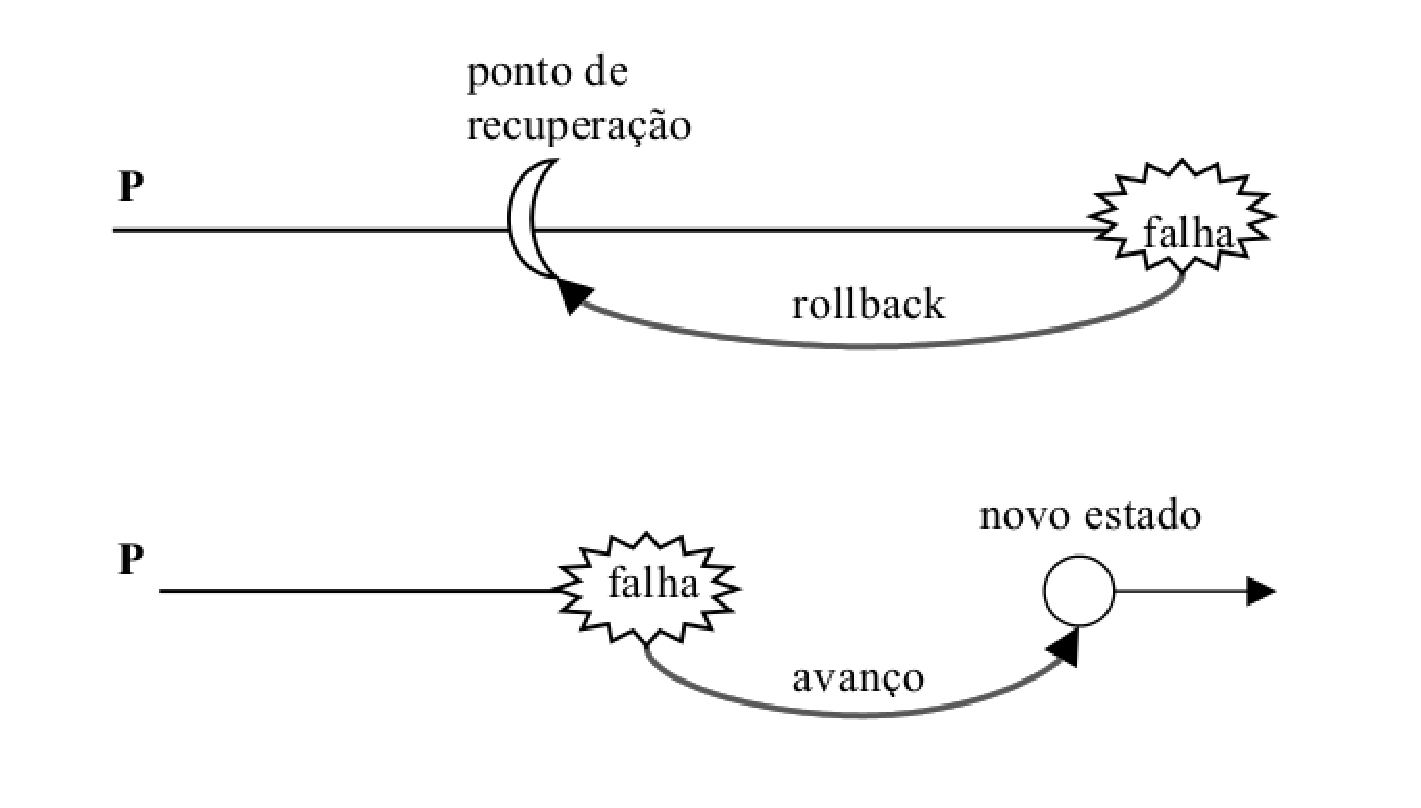
\includegraphics[height=200px]{img/recuperacao_ret_ava.eps}
% \caption{Recuperação por retorno e por avanço.}
% \label{fig:recuperacao_ret_ava}
%\end{figure}
% exemplo referencia: \ref{fig:recuperacao_ret_ava}

\begin{itemize}
 \item Detecção: a detecção de erro faz o monitoramento e aguarda uma falha se manifestar na forma de erro, para então
 passar para a próxima fase. Um exemplo de detecção de erro é o esquema de duplicação e comparação, onde é feita replicação do componente
 que realiza as operações sobre os mesmos dados e compara os resultados de saída. Caso ocorra alguma diferença nos resultados um erro é gerado.
 \item Confinamento: esta fase é responsável pela restrição de um erro para que esse não se propague para todo o sistema, pois entre a falha e a
 detecção do erro há um intervalo de tempo. Neste intervalo pode ocorrer a propagação do erro para outros componentes do sistema, por isso 
 antes de executar medidas corretivas é necessário definir os limites da propagação.
 \item Recuperação: após a detecção de um erro ocorre a recuperação, onde o estado de erro é alterado para estado livre de erros. A recuperação
 pode ser feita de duas formas:
 \begin{itemize}
  \item \textit{forward error recovery} ou recuperação por avanço: ocorre uma condução para um novo estado não ocorrido anteriormente. É o mais 
  eficiente, porém complexo de ser implementado pois a ação deve ser precisa.
  \item \textit{backward error recovery} ou recuperação por retorno: ocorre um retorno para um estado anterior que deve estar livre de erros.
  Para retornar ao estado anterior pode ser utilizado pontos de recuperação (\textit{checkpoints}), e quando ocorrer um erro, um \textit{rollback} 
  é executado, assim retornará a um \textit{checkpoint} anterior.
 \end{itemize}
 \item Tratamento: a última fase serve para prevenir que futuros erros aconteçam. Nesta fase ocorre a localização da falha para descobrir o 
 componente que originou a falha e após é feito um diagnóstico sendo que a remoção do componente danificado pode ser feita de duas formas, 
 manual ou automática. O reparo manual é feito por um operador, e o automático quando existe um componente em espera para substituição.
 Exemplo de um reparo manual é um operador fazer a troca de um disco de um servidor. E um exemplo de reparo automático é um disco configurado
 como \textit{hot spare}, que de acordo com \cite{rouse2013} \textit{hot spare} é definido como um componete de \textit{backup} que assumirá 
 o lugar de outro imediatamente após o componente principal falhar. Em \textit{storages} ou servidores a \textit{hot spare} pode ser configurada 
 em uma \textit{redundant array of independent disks} (RAID) juntamente com o \textit{array} de discos.
\end{itemize}

\section{Redundância}
\label{section:redundancia}

Redundância pode ser feita através da replicação de componentes, para reduzir o número de SPOF e garantir o mascaramento de falhas.
Na prática, se um componente falhar ele deve ser reparado ou substituído por um novo, sem que haja uma interrupção no serviço.
A redundância também pode ser através do envio de sinais ou \textit{bits} de controle junto aos dados, 
servindo assim para detecção de erros e até para correção \cite{weber2002}.

Segundo \cite{norvag2000} existem quatro tipos diferentes de redundância que são:
\begin{itemize}
 \item \textit{Hardware}: utiliza-se a replicação de componentes, sendo que caso um falhe outro possa assumir seu lugar. 
 Para fazer a detecção de erros a saída de cada componente é constantemente monitorada e comparada à saída de outros componentes.
 Um exemplo prático de redundância de \textit{hardware} é servidores com fontes redundantes, normalmente são duas fontes ligadas em paralelo, 
 caso uma falhe a outra suprirá a necessidade de todo o servidor;
 \item Informação: ocorre quando uma informação extra é enviada ou armazenada para possibilitar a detecção e correção de erros.
 Um exemplo clássico são os \textit{checksums} (soma de verificação). Esses são calculados antes da transmissão ou armazenamento 
 e recalculado ao recebê-los ou recuperá-los, assim sendo possível verificar a integridade dos dados. Outro exemplo bastante comum são os 
 \textit{bits} de paridade que são utilizandos para detectar falhas simples, que afetam apenas um \textit{bit} \cite{weber2002};
 \item \textit{Software}: redundância de \textit{software} não é muito útil pois replicando um \textit{software} as falhas ou 
 \textit{bugs} estarão presentes em todas replicas. Existem algumas técnicas que podem ajudar com esse problema. Por exemplo, programação 
 de n-versões, esta técnica consiste em criar n versões para um mesmo \textit{software} assim possibilitando o aumento da disponibilidade do 
 \textit{software}. Porém a programação de n-versões possui um custo muito elevado pois é complexo de manter. Além disso existem \textit{softwares} 
 para detecção de falhas, que muitas vezes podem ser utilizandos para detecção de falhas em \textit{hardware} também. Como por exemplo 
 um cão de guarda (\textit{watchdog timer}), ele recebe um sinal do programa ou serviço monitorado e caso este sinal não seja recebido, 
 devido alguma falha, o \textit{watchdog} irá fazer uma ação de reinicialização do serviço.
 \item Tempo: este é feito através da execução de instruções várias vezes no mesmo componente, assim detectando falha caso ocorra.
 Essa técnica necessita tempo adicional, e é utilizado onde o tempo não é crítico. Por exemplo um \textit{software} de monitoramento de serviços e
 servidores, ele faz o teste de cada serviço e caso ocorra uma falha o \textit{software} poderá executar uma ação corretiva para reestabelecer o
 serviço. Diferentemente de redundância de \textit{hardware} e informação ela não requer um \textit{hardware} extra para sua implementação 
 \cite{costa2009}.
\end{itemize}

\section{Cálculo da alta disponibilidade}

Um ponto importante sobre alta diponibilidade é como medi-la. Para isso são utilizados os valores de \textit{uptime} e 
\textit{downtime}, que são respectivamente o tempo que os serviços estão funcionando normalmente e o tempo que não estão funcionando.
Outra forma de expressar a alta disponibilidade é pela quantidade de ``noves'', isto é, se um serviço possui 4 noves de disponibilidade
este possui uma disponibilidade de 99,99\% \cite{pereirafilho2004}.

\begin{table}
\caption {Níveis de alta disponibilidade e exemplos de sistemas}
\label{tab:dispniveis}
\begin{center}
\begin{tabular}{|l|l|l|l|}\hline
Nível & Uptime & Downtime por ano & Exemplos\\\hline
1 & 90\% & 36.5 dias & computadores pessoais\\\hline
2 & 98\% & 7.3 dias & \\\hline
3 & 99\% & 3.65 dias & sistemas de acesso\\\hline
4 & 99.8\% & 17 horas e 30 minutos & \\\hline
5 & 99.9\% & 8 horas e 45 minutos & provedores de acesso\\\hline
6 & 99.99\% & 52.5 minutos & CPD, sistemas de negócios\\\hline
7 & 99.999\% & 5.25 minutos & sistemas de telefonia ou bancários\\\hline
8 & 99.9999\% & 31.5 minutos & sistemas de defesa militar\\\hline
\end{tabular}
\end{center}
\end{table}

A Tabela \ref{tab:dispniveis} possui alguns níveis de disponibilidade enumerados, seguido da porcentagem do \textit{Uptime} e 
o \textit{Downtime} por ano representado na medida de tempo.
Já a última coluna possui alguns exemplos de serviços relacionados ao nível de disponibilidade. 
Pode-se observar que para alguns serviços como sistemas bancários ou sistemas militares é necessário um alto nível de disponibilidade.

A alta diponibilidade pode ser calculada através da equação
\begin{equation}
d = \frac{MTBF}{(MTBF + MTTR)}
\label{diponibilidade}
\end{equation}
onde $d$ é a porcentagem de disponibilidade. O \textit{Mean Time Between Failures} ($MTBF$) é o tempo médio entre falhas, correspondendo ao 
tempo médio entre as paradas de um determinado serviço. Já o \textit{Mean Time To Repair} ($MTTR$) é o tempo médio de recuperação, isto é, 
o tempo entre a queda e a recuperação de um serviço \cite{goncalves2009}.

A alta disponibilidade é um dos principais fatores que fornece confiança aos clientes ou usuários, sendo extremante importante em empresas 
que fornecem serviços \textit{on-line}. Por isso existe o \textit{Service Level Agreement} (SLA), que é um acordo de nível de serviço, 
que garante que o serviço fornecido atenda as expectativas dos clientes. Um SLA é um documento contendo uma descrição e uma definição 
das características importantes do serviço que será fornecido. Esse acordo também deve conter o nível de serviço exigido pelo negócio, 
sendo que este deve ser minuciosamente definido. Por exemplo, um SLA pode conter descrição do serviço, requerimentos, horário de funcionamento,
disponibilidade esperada, entre outros \cite{smith2010}.

%\textit{Software} não possui falhas causadas por fatores físicos, ao contrário de \textit{hardware}.
%Falhas em \textit{software} são causadas por erros no seu desenvolvimento, resultando assim em ``\textit{bugs}'' que geralmente
%são causados por erros humanos. 
